\documentclass[12pt,twoside]{reedthesis}
\usepackage[utf8]{inputenc}
\usepackage{enumitem,amssymb,xcolor,cancel,gensymb,hyperref,graphicx,natbib}
\usepackage{graphicx,latexsym} 
\usepackage{amssymb,amsthm,amsmath}
\usepackage{longtable,booktabs,setspace}
\usepackage{aprilpreamble}

\usepackage[linesnumbered,ruled,vlined]{algorithm2e}
\SetKw{KwFrom}{from}

\usepackage{float}

\setlength{\parskip}{1em}

\bibliographystyle{plain}

\title{Unnamed Thesis}
\author{April Kopec}
\date{May 2024}

\division{Mathematics and Natural Sciences}
\advisor{Ira Globus Harris and Leonard Wainstein}
\department{Mathematics and Computer Science}

\begin{document}

\maketitle

\theoremstyle{definition}
\newtheorem{definition}{Definition}[chapter]



\mainmatter % here the regular arabic numbering starts
\pagestyle{fancyplain} % turns page numbering back on

%The \introduction command is provided as a convenience.
%if you want special chapter formatting, you'll probably want to avoid using it altogether

\onehalfspacing

    \chapter*{Introduction}
         \addcontentsline{toc}{chapter}{Introduction}
	\chaptermark{Introduction}
	\markboth{Introduction}{Introduction}
Neural networks have become a fundamental tool in the field of machine learning. But despite the fact that the lower-level implementation of a neural network is relatively simple, the behavior of neural networks has proven very difficult to analyze at a higher level. It has been estimated that GPT-4, a state-of-the-art large language model, has over one trillion parameters—though OpenAI has not officially disclosed the precise number. The neural networks used in the modern day contain vast amounts of data, and use that data in an opaque enough manner that the field has struggled to understand much about their behavior.

One possible avenue for understanding neural networks better is to analyze the relationship between the data they are trained on and their end behavior. What predictions can we make about how the final model would have been different if it had been trained on different data? \textit{Influence functions} are one approach through which we can try to answer this question.

At a high level, the idea behind an influence function is to calculate how much a very small change in the weighting of one training data point influences the resulting model. To discuss influence functions in more depth, we will first introduce some fundamental ideas in machine learning. These include parametric models, loss functions, and gradient descent.

\section{Parametric Models}
Suppose we have some data and want to produce a computer algorithm which can answer questions about our data. For instance, we might try to predict test performance based on how long someone spent studying, or someone's wealth based on their age. More usefully, a credit bureau might calculate your credit score (meant to measure likelihood of defaulting on loans), or an LLM might try to predict the next batch of characters based on the previous characters. An algorithm designed for this sort of task can be referred to as a ``predictive model"—by using some input data, the model makes a prediction about a related variable.

But how does one decide on the best model to use when dealing with some prediction task? This can be done using \textit{training data}, or a large collection of examples of input data the model might receive and the corresponding desired outputs. A training data set can be thought of as a series $\cl{D} = \Set{(x_i, y_i)}$ consisting of pairs of input data $x_i \in \cl{X}$ and outputs $y_i \in \cl{Y}$.

However, merely choosing whichever function $M: \cl{X} \to \cl{Y}$ is best at predicting the training data would not work well. A model which only memorizes a lookup table of which $y_i$ corresponds to which $x_i$ in the training data would perform perfectly during training, but would be nearly useless in practice. Our model should generalize to inputs outside of the training data, rather than only being effective on the exact examples it has already seen. (When a model fails to achieve this, it is known as \textit{over-fitting}.)

Instead, we can choose a function from a \textit{parameterized family of models}. The hope is that we can specify a family of models which use parameters $\theta_1, \theta_2, \cdots$ in a fixed manner to produce predictions. By confining the model to a particular form, we hope that it will have to learn generalizable properties about the training data, rather than just memorizing the specific training examples.

\begin{definition}
A \textbf{model} is a function $M: \cl{X} \to \cl{Y}$. The inputs $x \in \cl{X}$ can be thought of as collections of data about some question, and the outputs $M(x) \in \cl{Y}$ can be thought of as the model's answer. A \textbf{parameterized family of models} consists of a set $\cl{M}$ of models, a \textit{parameter space} $\Theta$, and a function which specifies a model $M_\theta \in \cl{M}$ given parameters $\theta \in \Theta$. If we have specified a family, we can use $M_\theta(x)$ to denote the output of the model specified by parameters $\theta$ when receiving the input $x$. If a model is a member of a parameterized family, it can be called a \textbf{parameterized model}.\cite{taboga21}
\end{definition} 

It is often reasonable to assume that $\cl X, \cl Y,$ and $\Theta$ are finite-dimensional vector spaces over $\R$—later, we will be applying vector calculus. (Though also note that sometimes it makes more sense to only consider a subset of the vector space. For example, if $y \in \cl Y$ is meant to represent a probability distribution over a discrete set, the components of $y$ ought to sum to one.)

This definition is fairly abstract, so it may be helpful to consider a few concrete examples.
\begin{enumerate}
    \item In simple linear regression, the model aims to predict some (real) number $y$ using a linear function of another number $x$. We do this using a models of the form $y = \beta_0 + \beta_1 x$. Here, $\beta_0$ can be interpreted as the \textit{intercept}, and $\beta_1$ can be interpreted as the \textit{slope}. In this case, $\cl X$ is $\R$, $\cl Y$ is $\R$, and $\Theta = \R^2$ contains vectors of the form $\theta = (\beta_0, \beta_1).$
    \item Linear regression can be generalized to multiple linear regression, where $\cl X = \R^n$. In this case, we have $y = \beta_0 + \beta \cdot x$, and $\Theta = \R \times \R^n$. Going further in the same direction, it can be generalized to to multivariate linear regression, where $\cl Y = \R^m$, $y=\beta_0 + Bx$ for a matrix $B$, and $\Theta = \R^m \times \cl M_{n \times m}$. A great many other generalizations are possible.
    \item In logistic regression, we try to estimate the probability of some event $Y$ based on a real number $x$. We use models of the form $\P[Y] = \dfrac{e^{\beta_0 + \beta_1 x}}{1 + e^{\beta_0 + \beta_1 x}}$. In this case, $\cl X = \R$, $\cl Y = (0, 1)$, and $\Theta = \R^2$. In logistic regression, it is still possible to think of $\cl Y$ as a vector space; you can have the model instead output $\logit(\P[Y]) = \ln\dfrac{\P[Y]}{1-\P[Y]} = \beta_0 + \beta_1 x$. Much like linear regression, logistic regression has several possible generalizations.
    \item Neural networks are too complicated to express using a simple equation, but the set of neural networks (of a fixed size) is a parametric family. For a neural network, $\cl{X}$ is a vector space where each component of $x$ is the activation of a neuron in the input layer, $\cl{Y}$ is the same for the output layer, and $\Theta$ contains large vectors whose components each represent one weighting of a connection between neurons. If you hear someone refer to the ``parameter count" of a neural network, they are referring to $\dim \Theta$ (or equivalently to the number of entries of a vector $\theta \in \Theta$.)
\end{enumerate}

From the breadth of the examples, it is clear that this is a very general framework. % Elaborate?

\section{Training Models}
\subsection{Loss Functions}
Given a parameterized family of models, we now need a method of selecting the best model. A first guess at an approach might be to choose the model that makes the most correct predictions when applied to the training data. However, typically we also care about answers that are \textit{approximately} correct, not only about answers that are exactly correct. This means that to choose the best model, we need some method of ``scoring" them which accounts for not just whether an answer is correct, but also how close it is to being correct. In machine learning, such a scoring method is referred to as a \textit{loss function}.

% I'm kind of unsatisfied with how I handle the distiction between a loss function for the whole training data set vs the loss function on a particular point
% I think the right mindset to be understanding this through has something like "pointwise loss ought to be the same thing as model loss on a database of size 1" as a key component
\begin{definition}
    Let $\fk D = \cl{P}(\cl{X} \times \cl Y)$ be the set of possible databases $\cl{D}$ of pairs $z_i = (x_i, y_i)$. A \textbf{loss function} is a function $\cl{L}: (\fk{D} \times \Theta) \to \R$ where $\cl{L}_{\cl{D}}(\theta)$ represents how \textit{poorly} the model $M_\theta$ performs on the database $\cl {D}$ when it tries to predict the outcomes $y_i$ given $x_i$. (When working with a fixed data set $\cl D$, we can leave it implicit and simply refer to $\cl{L}(\theta)$.) A \textbf{pointwise loss function} is a function $\ell: ((\cl{X} \times \cl{Y}) \times \Theta) \to \R$ such that $\cl {L}$ is equal to the average of $\ell$ across $\cl {D}$.
\end{definition}

It is often, though not necessarily, the case that the loss function is simply a measure of the quality of the model's predictions. For example, consider linear regression. Here, $\ell_{z_i}(\theta) = (M_\theta(x_i) - y_i)^2$, the squared error. In cases like this, $\ell_{z_i}(\theta)$ can be expressed as $d(M_{\theta}(x_i), y_i)$ where $d$ is some measure of prediction error.

Conversely, consider \textit{ridge regression}. Ridge regression is a modified form of linear regression which also tries to choose \textit{small} coefficients (or parameters), rather than just choosing whichever coefficients best predict the data. In the simplest case, ridge regression uses a loss function like \begin{equation*}
    \cl {L}(\theta) = \dfrac{1}{n}\Sum_{i=1}^n(M_\theta(x_i) - y_i)^2 + \lambda \Sum_j \theta_j^2,
\end{equation*}
where $\lambda$ is a factor which determines how strongly to penalize a larger coefficient. This loss function has one term for the mean squared error, and a second term which incentivizes the model to choose smaller parameters.

Equipped with the concept of a loss function, we can now express mathematically what the best parameters are for a given parametric family and a given training data set.

\begin{definition}
    Let $\theta^*$ be a tuple of parameters for a model $M$ in some parametric family with a given loss function $\cl{L}$ and training data set $\cl{D}$. The parameters $\theta^*$ are \textbf{globally optimal} if \begin{equation*}
        \theta^* = \displaystyle\argmin_{\theta \in \Theta} \cl{L}(\theta)
    \end{equation*}—that is, if there is no $\theta' \in \Theta$ such that $\cl{L}(\theta') < \cl{L}(\theta^*)$. If $\Theta$ has a topology, we say the parameters $\theta^*$ are \textbf{locally optimal} if there is a neighborhood of $\theta^*$ (imagine a region in $\Theta$ containing $\theta^*$ fully inside itself, rather than on the boundary) such that there are no better parameters $\theta'$ within that neighborhood.
\end{definition}
Informally, suppose we imagine parameters as being a horizontal position, and the loss for the corresponding model as being the elevation of the ground at that position. Then $\theta^*$ is a local optimum if it is the lowest point in some particular valley, and it is the global optimum if is in the deepest trench in the entirety of $\Theta$.

\subsection{Gradient Descent}
Given a parametric family, training data, and a loss function, how can you actually evaluate (or approximate) $\argmin_{\theta} \cl{L}(\theta)$ and select the optimal parameters? One common and effective technique is known as gradient descent. At a high level, the idea is to repeatedly update your parameters by a small step in whichever direction decreases loss the most.

\begin{definition}
Consider $\cl L$ as a scalar field over $\Theta = \R^p$ (that is, a function from $\Theta \to \R$). Then the \textbf{gradient} of $\cl L$ with respect to $\theta$ is given by
\begin{equation*}
    \nabla_\theta \cl{L} = \begin{bmatrix}\delf{}{\theta_1}\\ \vdots \\\delf{}{\theta_p}\end{bmatrix} \cl{L} = \begin{bmatrix}\delf{\cl{L}}{\theta_1}\\ \vdots \\\delf{\cl{L}}{\theta_p}\end{bmatrix}
\end{equation*}
where $\delf{\cl L}{\theta_i}$ is the partial derivative of $\cl L$ with respect to the $i$-th component of $\theta$. Because each partial derivative is a scalar field over $\Theta$, the gradient is a vector field.
\end{definition}

The key property of the gradient is that, for some fixed $\theta^*$, the gradient $\nabla_\theta \cl{L}(\theta^*)$ is a vector in $\Theta$ which points in the direction where a movement of $\theta^*$ \textit{increases} loss the quickest. Since the goal is to \textit{minimize} cost, we will instead be interested in the opposite direction, which is given by $-\nabla_\theta \cl L(\theta^*)$.

The process of gradient descent is described by the following pseudocode:

\begin{algorithm}[H]
    \caption{Gradient Descent}
    \For{$i$ \KwFrom $1$ \KwTo $\dim \Theta$}{
        Approximate $\delf{\cl L}{\theta_i}(\theta^*)$ by $\dfrac{\cl{L}(\theta^* + \frac{\epsilon}{2}e_i) - \cl{L}(\theta^* - \frac{\epsilon}{2}e_i)}{\epsilon}$
    }
    Calculate $\nabla_\theta \cl{L}(\theta^*)$ using partial derivatives\\
    Set $\theta^*$ to $\theta^* - \nabla_\theta\cl{L}(\theta^*)\delta$\\
    Repeat
\end{algorithm}
where $e_i$ is the basis vector in the $\theta_i$ direction, and $\epsilon$ and $\delta$ are small positive reals. The variable $\delta$ is sometimes known as the \textit{learning rate}.

This algorithm can be altered in many ways to make it more efficient—for example, lowering the learning rate $\delta$ over time as the model starts needing smaller refinements. But the high-level concept is always simply to follow the (negative) gradient down and hopefully approach a minimum.

\section{Influence Functions}
Suppose we want to consider how altering the training database $\cl D$ impacts the resulting model—in particular, we will consider \textit{local} alterations, rather than large ones. For this, it will be helpful to define the concept of a \textit{weighted} data set.

\begin{definition}
    A \textbf{weighted data set} $\cl D$ is a sequence $\Set{(z_i, w_i)}$ of data points $z_i$ and associated weightings $w_i$. Conceptually, sums in an unweighted data set correspond to weighted sums, averages to weighted averages, etc:
    \begin{align*}
    \begin{array}{ccc}
        \sum f(z_i) & \textbf{corresponds to} & \sum w_i f(z_i)\\
        \dfrac{\sum f(z_i)}{n} & \textbf{corresponds to} & \dfrac{\sum w_i f(z_i)}{\sum w_i}
    \end{array}
    \end{align*}
    An unweighted data set can be thought of as a weighted data set where each $w_i$ is equal to $1$.
    
    It is often useful to consider $\cl D$ as though it assigns a weighting to every possible data point $(x, y) \in (\cl{X} \times \cl{Y})$. In these cases, we say that the database assigns a weighting of $w = 0$ to each point not in its sequence; including a point in the sequence but assigning it a weight of zero is equivalent to excluding it.
\end{definition}

Now let us fix a particular data point $z_m = (x_m, y_m)$, which will have some weighting $w_m$. Suppose we change the weighting by some increment $\epsilon$. If $z_m$ was already in the unweighted data set, then setting $\epsilon = -1$ would be equivalent to removing it; if it was not, then setting $\epsilon = 1$ would be equivalent to adding it.

For a fixed choice of training data set and $z_m$, we will consider how the final model changes as a result of changing $\epsilon$.

\begin{definition}
    Let $\cl{D}_\epsilon$ denote the weighted data set where $\epsilon$ has been added to $w_m$. Then the \textbf{response} of $\theta$ to $z_m$ is given by \begin{equation}
        R_{m}(\epsilon) = \argmin_{\theta \in \Theta} \cl{L}_{\cl{D}_\epsilon}(\theta) = \argmin_{\theta \in \Theta}\dfrac{\sum_{i=1}^n w_i \ell_{z_i}(\theta)}{\sum_{i=1}^n w_i}
    \end{equation}

    The response of a function $f$ to $z_m$ is given by $f \circ R_m$. In particular, we might consider the response of loss $\cl L_{\cl D}(R_m(\epsilon))$ or the response of predictions $M_{R_m(\epsilon)}$.
    \end{definition}

The response function can be thought of as a curve through $\Theta$ parameterized by $\epsilon$; the response of loss can be easily visualized as a two dimensional graph where the $x$-axis represents $\epsilon$ and the $y$-axis represents $\cl{L}$.

\begin{definition}
    The \textbf{influence} of $z_m$ on $\theta$ is the derivative of the response function, evaluated at $\epsilon = 0$.
    \begin{equation}
\cl I(z_m) = \left.\delfrac{\theta}{\epsilon}\right|_{\epsilon = 0}
\end{equation}
The influence of $z_m$ on a differentiable function $f$ of $\theta$ is the derivative of the response of $f$ to $z_m$ evaluated at $\epsilon = 0$. Using the chain rule, we can calculate:
\begin{equation}
    \cl{I}_f(z_m) = \left.\delfrac{(f \circ R_{z_m})}{\epsilon}\right|_{\epsilon = 0} = \delfrac{f}{\theta} \left.\delf{\theta}{\epsilon}\right|_{\epsilon = 0} = \delf{f}{\theta} \cl{I}(z_m)
\end{equation}
where $\frac{\del f}{\del \theta}$ is evaluated at $\theta = R_{z_m}(0)$ (which is simply the value of $\theta$ before any reweighting). Note that if $f$ is a scalar function of $\theta$, then $\frac{\del f}{\del \theta}$ is the same as the gradient $\nabla_\theta f$; if it is a vector function, then it is a Jacobian matrix.\cite{bae22}\cite{grosse23}\cite{koh20}
% I need to double check that I'm not mixing up row and column vectors anywhere
\end{definition}
If the response function is thought of as a curve through $\Theta$, then the influence function would be the tangent vector to that curve at $\epsilon = 0$; the influence function tells you the direction the curve is moving in at that point. If the curve is sufficiently straight, then the influence can be used to approximate the response function:
\begin{equation*}
    R_m(\epsilon) \approx R_m(0) + \cl{I}(z_m)\epsilon + O(\epsilon^2).
\end{equation*}
(This is simply a Taylor approximation.)

The influence of $z_m$ on pointwise loss $\ell_{(x_i, y_i)}$ or on the prediction $M_{\bullet}(x_i)$ for some particular data point can be thought of as measures of how much the training data point $z_m$ contributed to the model's prediction for that particular data.

% The formatting of this section is difficult to get right; hopefully the spacing will just end up working out better as I do more work on the thesis, but if not I'll need to think more about it.
\subsection{Example}
To help make this more concrete, let us look at a very basic example: simple linear regression. Let the input space $\cl X$ and output space $\cl Y$ both be $\R$. Linear regression models are of the form $y = m x + b$, so $\Theta = \R^2$ and $\theta = (m, b)$. Our data set $\cl D$ will consist of some data points $(x_i, y_i)$, and our loss function will be given by the squared error $\ell_{(x_i, y_i)}(m, b) = ((mx_i + b) - y_i)^2$.

Consider the data set $\cl D = \Set{(0,0), (1, 1.5), (2, 2)}$. The model we get with weighting each point equally is $y = 1x + 0.167$. We find that the influence of $(0,0)$ on $\theta$ is $\cl{I}(0,0) \approx (0.083, -0.13)$, that $\cl{I} (1,1.5) \approx (0.00093, 0.11)$, and that $\cl{I}(2, 2) \approx (-0.083, 0.028)$. 

This confirms what we expect: if you imagine adjusting the model slightly in the direction of one of these influences, you will find that the model predicts the data point in question slightly better at the cost of predicting the other two points slightly worse.

\begin{figure}[H]
    \centering
    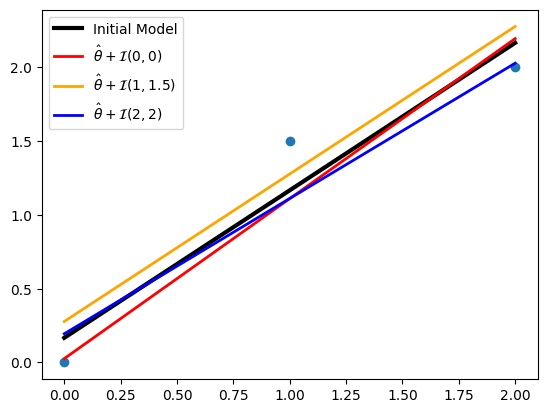
\includegraphics[width=0.5\linewidth]{example1.png}
    \caption{The three data points, along with four different models. The model in black is the model with equal weights. The other three models move the optimal model's parameters by one unit in the direction of $\cl{I}(z).$}
\end{figure}

We can also consider the influence on cost. We could calculate the influence of cost for any hypothetical data point anywhere in the $xy$ plane, but for now we will only use the training data points as our examples.

\begin{table}[H]
    \centering
    \begin{tabular}{c|c|c|c}
    & $\ell_{(0, 0)}$ & $\ell_{(1, 1.5)}$ & $\ell_{(2, 2)}$\\
    \hline
    $(0, 0)$ & $-0.046$ & $0.037$ & $0.009$\\
    \hline
    $(1, 1.5)$ & $0.037$ & $-0.074$ & $0.037$\\
    \hline
    $(2,2)$ & $0.009$ & $0.037$ & $-0.046$
    \end{tabular}
    \caption{The influence of the data points (rows) on the pointwise loss for each data point (columns). The symmetries are due to symmetries in the training data set.}
    \label{tab:my_label}
\end{table}

One thing to notice is how the influence of a data point on loss is negative for itself, but positive for other data points. This agrees with the notion that altering the parameters in the direction of the influence function for a data point improves prediction on that point (and others points which are well-predicted by similar parameters), potentially at the cost of others. We also see that the influence of a data point on the loss for itself is especially high.

\section{Future Work}
There are various issues with directly applying the influence function framework to deep learning techniques that are used in practice. The main current technique to adjust for them is by using the \textit{proximal Bregman response function} instead of the basic response function.\cite{bae22} I have been investigating how this works a bit, and have implemented the proximal Bregman objective in code, but I don't quite have a thorough understanding of them yet. I'd also like to apply these techniques to a more advanced example—maybe a neural network trained on MNIST.

There are a few details about the techniques Anthropic used in their recent paper which I don't have a very good grasp on yet. In particular, when they calculate which training data points were the most influential for some text completion, there is a step where they filter out the vast majority of the training data as uninfluential. I'd like to look more into what's going on there.\cite{grosse23}

I have not really come up with any great ideas for a novel research direction to pursue yet, and I would really like to find something like that to work on next semester, so I think that's a lot of what I will be focusing on in the coming weeks. I might spend some time looking through related robust statistics literature.
\bibliography{bibliography}
\end{document}

